\chapter{Marco teórico y Antecedentes }
\hrule \bigskip \vspace*{1cm}
%------------------------------------------------------------------------

\section{Desambiguación del sentido de las palabras (WSD)}
En general, la desambiguación del sentido de las palabras es el problema de seleccionar un sentido de un conjunto de posibilidades predefinidas para una palabra dada en un texto o discurso. 
En los últimos años se han incrementado las investigaciones para crear métodos de WSD. A continuación, se describe la clasificación para métodos de WSD de acuerdo a los recursos que utilizan (figura 2.1).

  \begin{figure}[h!]
	  \begin{center}
    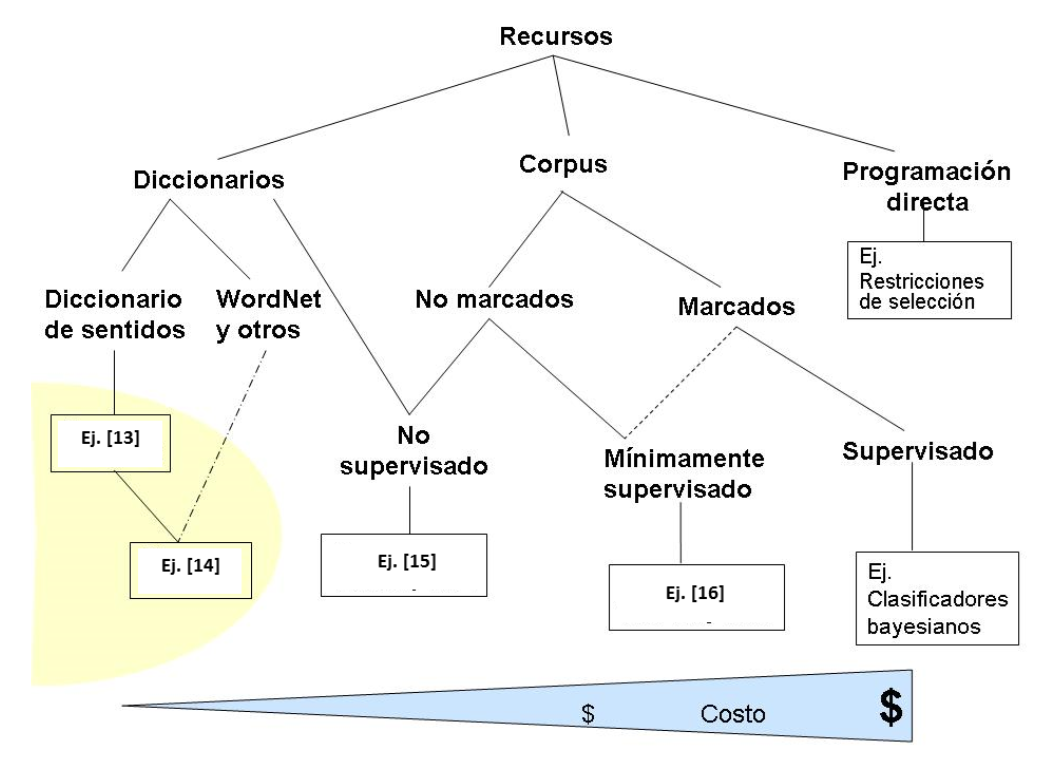
\includegraphics[angle=0, width=10cm]{Graficos/desambiguacion_WSD}
	  \caption{Clasificación de los métodos para WSD de acuerdo a los recursos que utilizan [1].}
    \end{center}
	\end{figure}

\section{Clasificación de sistemas en WSD}
\subsection{Métodos basados en conocimiento}
En esta categoría encontramos diferentes algoritmos para la etiquetación automática de sentidos. Normalmente, el rendimiento de estos métodos basados en conocimiento, es menor en comparación con los métodos basados en corpus. Pero con la salvedad de que los métodos basados en conocimiento tienen una amplia cobertura ya que pueden aplicarse a cualquier tipo de texto en comparación con los basados en corpus que sólo se pueden aplicar a aquellas palabras de las que se dispone de corpus anotados. A continuación, vamos a enumerar diferentes técnicas utilizadas por los métodos basados en conocimiento, aplicables sobre cualquier base de conocimiento léxica que defina sentidos de palabras y relaciones entre ellas. La base de conocimiento léxica más utilizada es WordNet (Miller (1995)). Vamos a describir 4 tipos diferentes de métodos basados en conocimiento:

\begin{itemize}
  \item Algoritmo de Lesk
  \item Similitud semántica
  \item Preferencias de selección
  \item Métodos Heurísticos
\end{itemize}

\subsubsection{Algoritmo de Lesk}
El algoritmo de Lesk [2] es uno de los primeros algoritmos exitosos usados en la desambiguación de sentidos de palabras. Este algoritmo se basa en dos puntos principales: un algoritmo de optimización para WSD y una medida de similitud para las definiciones de los sentidos.
El primer punto es acerca de desambiguar palabras considerando la coherencia global del texto, esto es, encontrar la combinación de los sentidos que maximice la relación total entre los sentidos de todas las palabras. 
Por ejemplo, para la oración \textit{My father deposits his money in a bank account} y considerando a lo más tres sentidos (véase tabla 1), para cada palabra, la figura 2 muestra la representación gráfica del algoritmo original de Lesk.

  \begin{figure}[h!]
    \begin{center}
    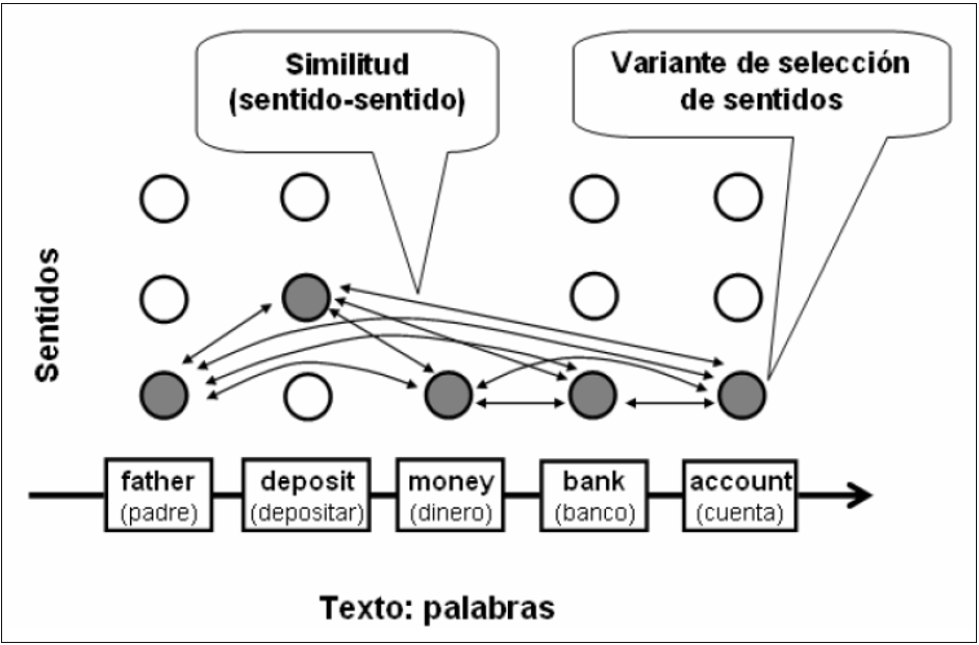
\includegraphics[angle=0, width=10cm]{Graficos/algoritmo_lesk}
    \caption{Representación gráfica del algoritmo original de Lesk [1]}
    \end{center}
  \end{figure}

  Tabla 1. Sentidos de las palabras (máximo tres) obtenidas de WordNet para la oración \textit{“My father deposits his money in a bank account”}.[1]

  \begin{table}[t]
    \centering
    \begin{tabular}{|m{2cm}|m{10cm}|}
    \hline
    % after \\: \hline or \cline{col1-col2} \cline{col3-col4} ...
    Palabra & Sentidos\\
    \hline
    \hline
    Father & 1: a male parent (also used as a term of address to your father); "his father was born in Atlanta". 
    2: `Father' is a term of address for priests in some churches (especially the Roman Catholic Church or the Orthodox Catholic Church); “`Padre' is frequently used in the military”. 
    3: a person who holds an important or distinguished position in some organization; "the tennis fathers ruled in her favor"; "the city fathers endorsed the proposal".\\
    \hline
    Deposit & bf \\
    \hline
    Money & bf \\
    \hline
    Bank & bf \\
    \hline
    Account& bf \\
    \hline
  \end{tabular}
    \caption{Como hacer una tabla}\label{tab:demo}
  \end{table}

\subsubsection{Similitud semántica}
\subsubsection{Preferencias de selección}
\subsubsection{Métodos Heurísticos}
\subsection{Métodos basados en corpus no supervisados}
\subsection{Métodos basados en corpus supervisados}
\subsection{Métodos híbridos}
%La forma como colocar un algoritmo es mediante el
%\verb"\usepackage{algorithmic}" y \verb"{algorithm}" este imprime de
%la siguiente forma:

\bigskip
\begin{algorithm}
\caption{Mapeamiento}\label{mapeadoEVA} processo\_ID(Identificación de flags)\\
Require: Lista de ${1\ldots N}$ que contenga los ID de las clases
correspondientes(provenientes del $FM$).
\begin{algorithmic} [1]
\STATE Generar \emph{lista} a partir de pares correspondientes según
$FM$ \WHILE {SchemaB contenga alguna clase}
\IF{valorASIG(\emph{claseB}) $\geq$ parametro \verb"VAL"}\STATE
\emph{claseB} $\Longleftarrow$ siguiente clase de SchemaB \STATE
\emph{lista} $\Longleftarrow$ agregar los términos de \emph{claseB}
y su correspondiente \emph{claseA} \STATE valor
(\emph{lista$(A_{i},B_{j})$})=\verb"POS"=$1$ \ENDIF \ENDWHILE
\end{algorithmic}
\end{algorithm}

NOTA: Este package no viene incluido por default en el \LaTeX ni con
esta plantilla, pero si es de mucha utilidad, esta disponible en
internet así como muchas otras. Si desean incluir un nuevo
\verb"\usepackage{Nombre_Package}", solo deben agregarla en el
archivo \verb"unsa.cls" en una linea y ya estará disponible.

\begin{table}[h]
  \centering
  \begin{tabular}{|c|c|c|c|c|}
  \hline
  % after \\: \hline or \cline{col1-col2} \cline{col3-col4} ...
  Me & Sem & Lug & Pos & Gen\\
  & Cas & & &\\
  \hline
  \hline
  a & bf & sd & as & hj \\
  a & bf & sdff & fg & ert \\
  a & bf & as & fg & klj \\
  \hline
\end{tabular}
  \caption{Como hacer una tabla}\label{tab:demo}
\end{table}


\begin{figure}
\begin{center}

\includegraphics[angle=45, width=5cm]{Graficos/escuela}
\caption{Logotipo de la EPCC}
\end{center}
\end{figure}
